\documentclass[conference]{IEEEtran}
\IEEEoverridecommandlockouts
% The preceding line is only needed to identify funding in the first footnote. If that is unneeded, please comment it out.
\usepackage{cite}
\usepackage{amsmath,amssymb,amsfonts}
\usepackage{algorithmic}
\usepackage{graphicx}
\usepackage{textcomp}
\usepackage{xcolor}
\usepackage{url}
\usepackage{hyperref}
\usepackage{xurl}

\def\BibTeX{{\rm B\kern-.05em{\sc i\kern-.025em b}\kern-.08em
  T\kern-.1667em\lower.7ex\hbox{E}\kern-.125emX}}
\begin{document}

\title{Analyzing the Effects of Memory Pressure on Container and Virtual Machine Performance\\
% {\footnotesize \textsuperscript{*}Note: Sub-titles are not captured in Xplore and
% should not be used}
% \thanks{Identify applicable funding agency here. If none, delete this.}
}

\author{\IEEEauthorblockN{1\textsuperscript{st} Ravi Pandey}
\IEEEauthorblockA{\textit{Department of Computer Science} \\
\textit{University of Nebraska at Omaha}\\
Omaha, U.S.A. \\
ravipandey@unomaha.edu}
\and
\IEEEauthorblockN{2\textsuperscript{nd} Carson Cahoy}
\IEEEauthorblockA{\textit{Department of Computer Science} \\
\textit{University of Nebraska at Omaha}\\
Omaha, U.S.A. \\
carsoncahoy@unomaha.edu}
}

\maketitle

\begin{abstract}
Virtualization is one of the most important technologies used in cloud computing as containers and virtual machines (VMs) allow workload distribution across physical hardware in multiple ways. Containers provide lightweight isolation by sharing the host kernel, which can expose applications to performance degradation under memory pressure. On the other hand, VMs provide stronger isolation but it is at the cost of additional memory overhead. This project aims to investigate the effects of memory pressure on Docker containers and Kernel-based VMs (KVMs) by focusing on throughput, tail latency, and performance degradation under controlled memory, swap, and stress scenarios. By analyzing observed performance changes with Linux kernel memory management mechanisms, including cgroup limits, page reclaim policies, and Out-Of-Memory (OOM) behavior, the study will provide mechanism-level insights into resource isolation, multi-workload interference, and performance predictability. The results can inform best practices for deploying workloads in memory-constrained virtualized and containerized environments.
 
\end{abstract}

\begin{IEEEkeywords}
containerization, virtual machine, memory pressure, resource isolation
\end{IEEEkeywords}

\section{Introduction}

Virtualization is a core operating system concept which enables multiple isolated execution environments to share a single physical machine while maintaining abstraction of hardware resources. Classic operating systems literature describes virtualization as a mechanism for improving resource utilization, isolation, and system flexibility by multiplexing hardware among independent workloads \cite{silberschatz2018operating}. Modern computing platforms are heavily dependent on virtualization to support cloud computing, multi-tenant infrastructure, and scalable service deployment. Two primary virtualization approaches are virtual machines (VMs) and containers. Virtual machines emulate hardware and run independent guest operating systems under a hypervisor, providing strong isolation guarantees. In contrast, containers implement operating system-level virtualization by sharing the host kernel while isolating applications through namespaces and control groups, which enable lightweight deployment and high resource efficiency. Empirical studies show that both technologies enable efficient workload consolidation with near-native CPU and memory performance, although their overhead characteristics and isolation properties differ across workloads \cite{felter2015comparison}.

In this work, \textit{memory pressure} refers to conditions in which memory demand approaches or exceeds available physical memory, triggering reclaim or swapping. Linux control groups (cgroups) enforce per-container memory limits and track usage, enabling controlled reclamation and out-of-memory handling when limits are exceeded \cite{linux_cgroup_memory_controller}. \textit{Swapping} and \textit{page reclaim} refer to kernel mechanisms that evict memory pages to disk or free inactive pages to satisfy allocation requests. \textit{Tail latency} denotes high-percentile response times that capture worst-case delays and are critical for service-level objectives \cite{dean2013tail}. \textit{Resource fairness} describes proportional and predictable allocation of memory resources among competing workloads. In virtualized systems, memory reclamation may introduce \textit{double paging}, where both guest and hypervisor independently reclaim memory, increasing overhead and performance degradation \cite{WaldspurgerProceedingsOT}.

Memory pressure has become a critical systems challenge in virtualized environments due to increasing workload density and memory overcommitment practices. Overcommitment allows providers to increase utilization but may trigger reclaim activity, swapping, and thrashing when aggregate working sets exceed physical memory capacity \cite{nakazawa2017taming}. Under such conditions, performance becomes unpredictable as applications compete for limited memory resources, which leads to resource contention and degraded throughput. Prior work demonstrates that containerized workloads show significant performance loss and QoS violations under extreme memory pressure, particularly when Linux reclaim policies aggressively swap active pages \cite{nakazawa2017taming}. Moreover, modern services are highly latency-sensitive, which makes tail latency a critical performance metric, since even a small increases in memory stall times can lead to significant degradation in quality of service and user experience \cite{dean2013tail}. 

A central tension exists between containers and virtual machines in how they handle resource isolation under memory stress. Containers provide lightweight isolation and high efficiency by sharing the host kernel, but this shared kernel architecture can expose workloads to interference under contention. Virtual machines provide stronger isolation by virtualizing hardware resources, yet this isolation introduces additional memory overhead and complex reclamation interactions between guest and host memory managers. These differences raise important questions about performance degradation patterns and predictability when memory becomes scarce.

There are several key challenges that motivate this work. Memory pressure can lead to performance degradation through page reclaim, swapping, and cache eviction, increasing latency and reducing throughput. It becomes difficult to ensure fairness and resource isolation when multiple workloads compete for memory, especially in multi-tenant environments. Swap behavior and page reclaim policies may introduce significant overhead and I/O amplification. Additionally, multi-workload interference can cause noisy-neighbor effects, undermining performance guarantees even when resource limits are configured.

This project investigates the following research question: \textit{How does memory pressure influence performance and isolation in container-based versus virtualized environments?}

This project aims to provide a systematic evaluation of memory pressure effects in Docker containers and KVM virtual machines through controlled stress scenarios. Prior comparisons of containers and VMs have focused primarily on baseline performance and overhead \cite{felter2015comparison}. More recent work on container run-times highlights limitations in performance isolation under concurrent memory stress \cite{bhaia2024isolation}. Building on these findings, this study analyzes performance degradation and tail latency under memory stress, and performs a mechanism-level analysis of Linux memory management behavior, including cgroup enforcement, reclaim activity, swapping, and OOM handling. By linking observed performance behavior to underlying kernel mechanisms, the project seeks to provide actionable insights for deploying workloads in memory-constrained and multi-tenant environments.




\section{Background and Related Work}
%----------------------------------------------
Memory management under contention is a key challenge in virtualized and containerized systems, especially with the growing workload density in cloud systems that rely on memory overcommitting to achieve better resource utilization. The traditional operating systems literature defines memory management as a trade-off between efficiency and isolation, where memory allocation policies have to avoid interference while sustaining high utilization \cite{silberschatz2018operating}. This trade-off becomes difficult to achieve in multi-tenant scenarios where the aggregate workloads approach physical memory size.

Some early studies have established baseline performance characteristics of virtualization technologies. Felter et al. \cite{felter2015comparison} demonstrated that both Docker containers and KVM virtual machines achieve near-native CPU and memory performance, with some overhead arising from I/O subsystems and configuration choices. Because performance differences are small under normal conditions, later research has focused on behavior under contention and stress, where isolation guarantees and resource management policies become critical.

Recent studies show that performance isolation is still a challenge in containerized environments. Bhaia et al. \cite{bhaia2024isolation} evaluated multiple container run-times and found that concurrent memory-intensive workloads can lead to significant throughput degradation despite configured isolation mechanisms. Their results highlight trade-offs between efficiency and stronger sand-boxing approaches indicating that runtime design and kernel sharing influence interference patterns under contention.

A key factor driving interference is memory pressure, which triggers page reclaim and swapping. Under severe overcommitment, Linux reclaim policies may evict active pages and induce thrashing, causing disproportionate degradation among heavily utilized containers \cite{nakazawa2017taming}. This work demonstrates that reclaim policy parameters, such as swappiness, strongly influence performance isolation and that degradation thresholds are difficult to predict in highly overcommitted systems.

Memory pressure introduces additional complexity in virtual machine environments due to interactions between guest operating systems and hypervisors. ESX memory management framework introduced ballooning and share-based allocation to support overcommitment while preserving fairness \cite{WaldspurgerProceedingsOT}. Ballooning shifts reclamation decisions to the guest OS, which reduces inefficient hypervisor swapping and mitigating double paging. Experimental analysis confirms that ballooning generally has lower performance penalties than hypervisor-level swapping because the guest OS can reclaim less critical pages, such as buffer cache contents \cite{moniruzzaman2014ballooning}. These mechanisms show how VM-level reclamation policies influence degradation behavior under pressure.

Beyond static limits and reclaim strategies, adaptive memory control approaches have been proposed to improve stability. Nakagawa and Oikawa \cite{nakagawa2016behavior} introduce a behavior-based memory management method that monitors consumption growth and dynamically applies limits when abnormal usage is detected. Their results suggest that static limits alone may be insufficient to prevent degradation caused by rapid or anomalous memory consumption.

At the container level, the Linux memory cgroup controller provides the primary mechanism for enforcing limits and isolating memory usage. It tracks anonymous memory and page cache usage, performs local reclaim when limits are exceeded, and triggers out-of-memory handling when reclaim fails \cite{linux_cgroup_memory_controller}. Because reclaim decisions occur within the cgroup boundary, container performance can be strongly influenced by limit configuration and reclaim activity.

Understanding memory pressure effects requires controlled stress generation and reproducible workloads. Tools such as \textit{stress-ng} generate configurable memory and CPU pressure, enabling systematic evaluation of reclaim behavior \cite{stressng}. The \textit{memhog} utility allocates and faults memory deterministically, allowing controlled experiments on allocation pressure and locality effects \cite{memhog_manpage}. Additionally, the Flexible I/O Tester (\textit{fio}) can create page-cache pressure and swapping through controlled storage workloads for analysis of interactions between memory pressure and I/O activity \cite{fio2023}. These tools support repeatable experiments that isolate memory contention effects.

Latency sensitivity further amplifies the importance of understanding memory pressure. Dean and Barroso emphasize that tail latency dominates user-perceived performance in large-scale services, where small increases in stall time can significantly degrade responsiveness \cite{dean2013tail}. Memory reclaim, swapping, and cache eviction can introduce unpredictable stalls, making high-percentile latency a critical metric when evaluating system behavior under pressure.

Despite extensive research on virtualization overhead, container isolation, and memory overcommitment, important gaps remain. Existing studies often examine containers or virtual machines independently, focus on extreme overcommitment scenarios, or emphasize throughput rather than fairness and predictability. A systematic, mechanism-aware comparison of containers and virtual machines under controlled memory pressure, linking performance degradation, tail latency, and fairness to underlying memory management behavior, remains limited.

This work aims to address these gaps by combining controlled stress scenarios, multi-workload contention experiments, and analysis of kernel and hypervisor memory management mechanisms. By examining reclaim activity, swapping behavior, cgroup enforcement, and VM ballooning interactions, one of the study goals is to characterize degradation patterns and isolation properties in memory-constrained environments.

\section{Problem Definition}
To address these gaps, we define a controlled experimental model that enables systematic comparison of container-based and virtualized environments under memory pressure. This section of the paper defines the system model, memory pressure scenarios, performance, and metrics evaluated in this study.

We consider a single physical host equipped with fixed CPU, memory, and storage resources. On this host, workloads will be deployed using a container-based virtualization using Docker or hardware virtualization using Kernel-based Virtual Machines (KVMs). The objective of the project is to analyze and compare the results on how the two approaches respond to memory pressure under controlled and reproducible conditions.

In the container-based configuration, multiple containers share the host Linux kernel. Memory usage will be controlled by the use of Linux control groups (\textit{cgroups}), which enforce per container limits and trigger page reclaim, swapping, or OOM handling when limits are surpassed. Because containers share the same kernel and page cache, memory contention may result in interference between the workloads. 

In the virtual memory configuration, each KVM instance will run as its own guest operating system with a fixed memory allocation. Memory reclamation may occur at the hypervisor level or even at the guest level. This layered memory management can introduce additional overhead such as double paging, where both guest and host reclaim memory separately. VMs therefore provide stronger isolation but may result in higher reclamation cost under pressure.

Memory pressure can be defined as the condition in which total memory demand approaches or exceeds available physical memory. In the container-based experiments, memory pressure is defined relative to the cgroup memory limits imposed on each container. In contrast, for the KVM experiments, memory pressure is defined relative to the fixed memory allocation of the guest virtual machine. This ensures that pressure is evaluated within the relevant isolation boundary in each environment rather than at the host level, enabling a consistent comparison of container-level and VM-level memory behavior.

To enable systematic evaluation, we define three pressure regimes:

\begin{itemize}
\item \textbf{Moderate pressure:} aggregate memory usage approaches system capacity, triggering limited reclaim.
\item \textbf{High pressure:} demand exceeds available memory, causing aggressive reclaim and potential swap activity.
\item \textbf{Extreme pressure:} severe overcommitment leads to frequent reclaim activity, increased latency, and potential OOM events.
\end{itemize}
These three regimes allow for systematic evaluation of performance degradation, system stability and isolation behavior.

We will evaluate system behavior using the following criteria:

\begin{itemize}
\item \textbf{Throughput:} amount of useful work done per unit time.
\item \textbf{Tail latency:} high-percentile response times capturing worst-case delays.
\item \textbf{Performance degradation:} relative loss of throughput under contention compared to baseline.
\item \textbf{System stability indicators:} swap activity, major page faults, and OOM events.
\end{itemize}

\section{Methodology}
\subsection{Experimental Environment}
All experiments in this project are performed on a single Linux host machine running Ubuntu 22.04, which serves as both the Docker execution platform and the hypervisor for KVM experiments. The host system is equipped with 64\,GB of RAM and an Intel Core i7-7700T CPU.


Two environments are evaluated in this study. The container-based environment runs directly on the Linux host, while the virtual machine environment runs the same service and stress workload inside a KVM guest. Both environments use the same workload definitions, enabling direct comparison.

\subsection{Experimental Design}
This study uses a controlled benchmarking methodology to evaluate how memory pressure affects performance and isolation in both Docker containers and KVM guest environments. Both experiment tracks use the same workload structure and parameter sweep. In both cases, the study uses a single global baseline, fixed \texttt{ApacheBench (ab)} \cite{apachebench} concurrency, and the same set of memory-pressure levels.

For the Docker \cite{merkel2014docker} campaign, we run a service container and a stressor container on the same Linux host. The service is exposed on \texttt{127.0.0.1:8080}, “the stressor generates memory pressure, and ApacheBench is used to measure throughput and latency under swappiness values 10, 60, and 100 and stress levels moderate, high, and extreme. The Docker runs use one baseline configuration at swappiness 60, followed by the stressed matrix with three repeats per configuration. 

% The run order, output naming, and repeat handling are controlled by the scripts in \texttt{experiments/configs.sh}, \texttt{experiments/run\_base.sh}, \texttt{experiments/run\_one.sh}, and \texttt{experiments/run\_matrix.sh}.

For the KVM \cite{kivity2007kvm} campaign, we follow the same matrix structure inside a Linux virtual machine. The guest runs a lightweight HTTP service, a memory stressor generated with \textit{stress-ng}, and ApacheBench against \texttt{http://127.0.0.1:8080/}. 
% The guest runbook in \texttt{kvm\_experiments/KVM\_SETUP\_LINUX.md} documents the VM creation and validation steps used for this setup.

The goal is to compare how memory pressure affects throughput, latency, and system stability under different isolation mechanisms. The scripts record application metrics together with kernel-level snapshots so that observed slowdowns can be tied to reclaim, swapping, and out-of-memory behavior \cite{linux_oom} \cite{linux_vm_sysctl}.

Experiments are defined by fixed configurations of memory limits, pressure levels, and kernel parameters. Automated scripts execute the full experimental matrix and collect system-level metrics.

\subsection{System Architecture Overview}

To clarify the experimental setup and workload interactions, Figure ~\ref{fig:architecture} illustrates the system architecture for both the container-based and virtual machine-based environments.

In the Docker-based setup, the ApacheBench (AB) client sends HTTP requests to a latency-sensitive service running inside a container. A separate container runs a memory-intensive stress workload using \textit{stress-ng}. Both containers share the host Linux kernel and compete for memory resources through cgroup-enforced limits \cite{linux_cgroup_memory_controller}.

In the KVM-based setup, the ApacheBench client sends requests to a service running inside a virtual machine. Within the VM, both the service and the stress workload execute under the guest operating system. Memory pressure is therefore handled within the VM boundary, and the host kernel does not directly mediate contention between the service and stressor. This provides stronger isolation compared to containers but limits direct resource sharing.
\begin{figure}[t]
\centering
\includegraphics[width=0.95\columnwidth]{images/setup__.png}
\caption{System architecture for Docker (top) and KVM (bottom) experimental setups.}
\label{fig:architecture}
\end{figure}

\subsubsection{Container Environment}
In the container-based configuration, workloads are deployed using Docker containers on the host Linux system \cite{merkel2014docker}. The service runs in one container and the memory stressor runs in another container on the same host. Containers use \textit{cgroups} \cite{linux_cgroup_memory_controller} to enforce memory limits. Memory limits are configured using Docker runtime flags:

\begin{itemize}
\item \texttt{--memory} to restrict container memory usage
\item \texttt{--memory-swap} to control swap availability
\end{itemize}

Each experimental run launches two containers:

\begin{itemize}
\item \textbf{C1}: latency-sensitive service container
\item \textbf{C2}: memory stressor container
\end{itemize}
This configuration allows the study of interference effects between competing workloads. The Docker scripts also record pre- and post-run \texttt{/proc/vmstat}, \texttt{/proc/meminfo}, and kernel OOM traces for each run.

\subsubsection{Virtual Machine Environment}

In the virtualized configuration, workloads are deployed inside a single KVM virtual machine managed through QEMU \cite{bellard2005qemu}. The guest runs an independent operating system with a fixed memory allocation.

Within the VM, two workloads are executed:

\begin{itemize}
\item \textbf{Service}: latency-sensitive HTTP service
\item \textbf{Stressor}: memory-intensive workload generated using \textit{stress-ng}
\end{itemize}

This configuration allows controlled evaluation of memory pressure within the VM environment.

\subsection{VM Resource Configuration and Constraints}

The KVM experiments were conducted using a guest virtual machine configured with 4\,GB of RAM and 2 vCPUs on a host system equipped with an Intel Core i7-7700T processor. 


\subsection{Workload Composition}

The experiments simulate a simplified multi-tenant cloud scenario consisting of two interacting workloads.

\subsubsection{Latency-Sensitive Service}

The primary workload is a lightweight HTTP service running inside the container or virtual machine. The service represents an application that is sensitive to latency degradation under resource contention.

Client requests are generated using \textit{ApacheBench (ab)} \cite{apachebench}, which produces high request concurrency and reports detailed throughput and latency metrics.

ApacheBench provides measurements including:

\begin{itemize}
\item requests per second
\item mean response latency
\item high-percentile latency (95th and 99th percentiles)
\end{itemize}

These metrics allow evaluation of both average performance and tail latency behavior, which is critical for latency-sensitive applications \cite{dean2013tail}.

\subsubsection{Memory Stressor}

Memory pressure is generated using the \textit{stress-ng} utility \cite{stressng}. The stressor allocates and faults memory pages continuously, simulating applications with high memory demand.

The stressor container or VM is configured to allocate memory at predefined levels corresponding to the pressure regimes defined earlier in the paper. This approach allows controlled generation of memory contention while maintaining repeatability. The memory allocations used in the current scripts are 400 MB for moderate pressure, 800 MB for high pressure, and 1200 MB for extreme pressure.

\subsection{Memory Pressure Regimes}

Experiments are conducted under three levels of memory pressure:

\begin{itemize}
\item \textbf{Moderate pressure}: memory usage approaches available system memory and triggers limited reclaim.
\item \textbf{High pressure}: memory demand exceeds available physical memory and triggers aggressive reclaim.
\item \textbf{Extreme pressure:} severe overcommitment leads to frequent reclaim activity, increased latency, and potential system instability.
\end{itemize}

The stress levels are implemented through configurable \texttt{stress-ng} parameters specifying memory allocation sizes and duration. Experiments also vary the Linux kernel parameter \texttt{vm.swappiness}.


Swappiness controls the kernel’s preference for swapping out anonymous memory versus reclaiming page cache. Different swappiness values influence reclaim aggressiveness and can significantly affect performance under memory pressure \cite{nakazawa2017taming}. In this study, the matrix uses swappiness values 10, 60, and 100 with a single global baseline at swappiness 60.

Memory pressure is defined relative to the available memory within each environment. This ensures comparable pressure conditions within each isolation boundary rather than at the host level.

\subsection{Mixed Workload Interference}

To analyze multi-tenant interference, the experiments colocate the latency-sensitive service with the memory stressor on the same host kernel or hypervisor.

This setup allows evaluation of scenarios such as:

\begin{itemize}
\item a memory-intensive workload degrading the latency of a neighboring service
\item increased reclaim activity causing latency spikes
\item memory pressure leading to swap activity or OOM events
\end{itemize}

By comparing isolated baseline runs with colocated runs, the study quantifies how much interference arises from memory contention \cite{mars2011bubble}.

\subsection{Measurement and Instrumentation}

The experiments collect both application-level metrics and kernel-level system metrics to enable mechanism-level analysis.

\subsubsection{Application-Level Metrics}

Application performance is measured using ApacheBench output. The following metrics are collected:

\begin{itemize}
\item \textbf{Throughput}: requests per second
\item \textbf{Mean latency}
\item \textbf{Tail latency} (95th and 99th percentiles)
\end{itemize}

Tail latency is particularly important because memory reclaim and swapping can introduce long response delays.

\subsubsection{Kernel-Level Metrics}

System-level metrics are collected from Linux \texttt{/proc} interfaces and kernel logs \cite{linux_vm_sysctl}.

Key metrics include:

\begin{itemize}
\item \texttt{/proc/meminfo} -- overall memory usage
\item \texttt{/proc/vmstat} -- page fault and swap activity
\item major page faults (\texttt{pgmajfault})
\item swap-in events (\texttt{pswpin})
\item swap-out events (\texttt{pswpout})
\item kernel logs (\texttt{dmesg}) for OOM events
\end{itemize}


Although swap activity is monitored, preliminary observations indicate that most configurations do not exhibit sustained swap-in or swap-out activity. Therefore, performance degradation is expected to be driven primarily by memory reclaim and contention rather than heavy swapping.

\subsubsection{OOM Behavior Monitoring}

Out-of-memory events are captured using kernel log \cite{linux_oom}. In container environments, OOM handling may occur at two levels:

\begin{itemize}
\item \textbf{Cgroup-level OOM}, where the kernel kills a process within a container whose memory limit is exceeded.
\item \textbf{Host-level OOM}, where the system-wide OOM killer terminates processes when overall memory exhaustion occurs.
\end{itemize}

Understanding which mechanism is triggered helps explain differences in isolation behavior between containers and VMs.

\subsection{Performance Degradation Metrics}

Performance degradation is evaluated using proportional slowdown \cite{hennessy2017computer}, which measures how much a workload’s performance changes relative to its isolated baseline:

\[
slowdown_i = \frac{T_{baseline}}{T_{contended}}
\]

where $T_{baseline}$ is the standalone throughput and $T_{contended}$ is the throughput under contention.

This metric captures the relative impact of memory pressure on application performance and allows comparison across different configurations and environments. In this study, proportional slowdown is used as the primary indicator of performance degradation under memory pressure.

\subsection{Experimental Automation and Data Analysis}

Experiments are fully automated using scripts that configure and execute workloads, iterate over stress levels and kernel parameters, and record results. Each Docker or KVM run generates a dedicated results directory containing benchmark output, kernel snapshots, and OOM logs. Multiple repetitions of each configuration are performed to account for variability, and results are aggregated. The current scripts use three repetitions per stressed configuration.

Collected data is analyzed to relate memory pressure, kernel behavior, and application performance. Proportional slowdown relative to baseline is computed, and kernel metrics (page reclaim, swap activity, major page faults, and OOM events) are examined to identify sources of degradation. Container and VM environments are compared to evaluate how isolation mechanisms influence performance under memory pressure.

In some high-pressure configurations, transient failures such as socket connection resets were observed during benchmarking. These cases were rerun to obtain valid measurements. Such failures are treated as part of system behavior under extreme memory pressure rather than experimental errors.

\subsection{Rationale for Methodological Choices}

The experimental methodology was chosen to provide a mechanism-aware evaluation of memory pressure effects in virtualized environments.

Several design choices support this goal:

\begin{itemize}
\item Controlled stress generation enables reproducible memory pressure scenarios.
\item Latency-sensitive HTTP workloads allow measurement of tail latency effects that are often hidden in average performance metrics.
\item Kernel-level instrumentation provides visibility into reclaim, swap, and OOM events that explain performance degradation.
\item Parallel container and VM configurations enable direct comparison of isolation properties between lightweight and hardware virtualization.
\end{itemize}

These techniques enable the study to connect high-level application behavior with low-level kernel mechanisms, which addresses the research question of how memory pressure influences performance and isolation.

\subsection{External Tools and Platforms}

The following external tools are used in this study:

\begin{itemize}
\item \textbf{Docker}: container runtime providing namespace and cgroup-based isolation
\item \textbf{KVM/QEMU}: hardware-assisted virtualization framework for running virtual machines
\item \textbf{stress-ng}: configurable system stress-testing tool used to generate memory pressure \cite{stressng}
\item \textbf{ApacheBench (ab)}: HTTP benchmarking tool used to measure throughput and latency
\end{itemize}

These tools were selected because they are widely used in systems research and allow precise control over workload characteristics.
\section{Results}

This section presents experimental results for both Docker and KVM environments, focusing on throughput, tail latency, and performance degradation under varying memory pressure conditions. For most summary plots, markers indicate the mean across three runs, with error bars showing the standard deviation where available. Additionally, a distribution plot shows all individual runs to illustrate run-to-run variability.

\subsection{Docker Experiments}

The Docker campaign used a single global baseline at swappiness 60 and a fixed ApacheBench concurrency of 30 across all baseline and stressed runs. The completed dataset contains three repeats for each stressed configuration, and the summary files confirm that the experiment matrix executed as intended. The most relevant plots are shown in Figures~\ref{fig:docker-slowdown}, \ref{fig:docker-throughput}, \ref{fig:docker-tail}, and \ref{fig:docker-heatmap}.

\begin{figure}[t]
  \centering
  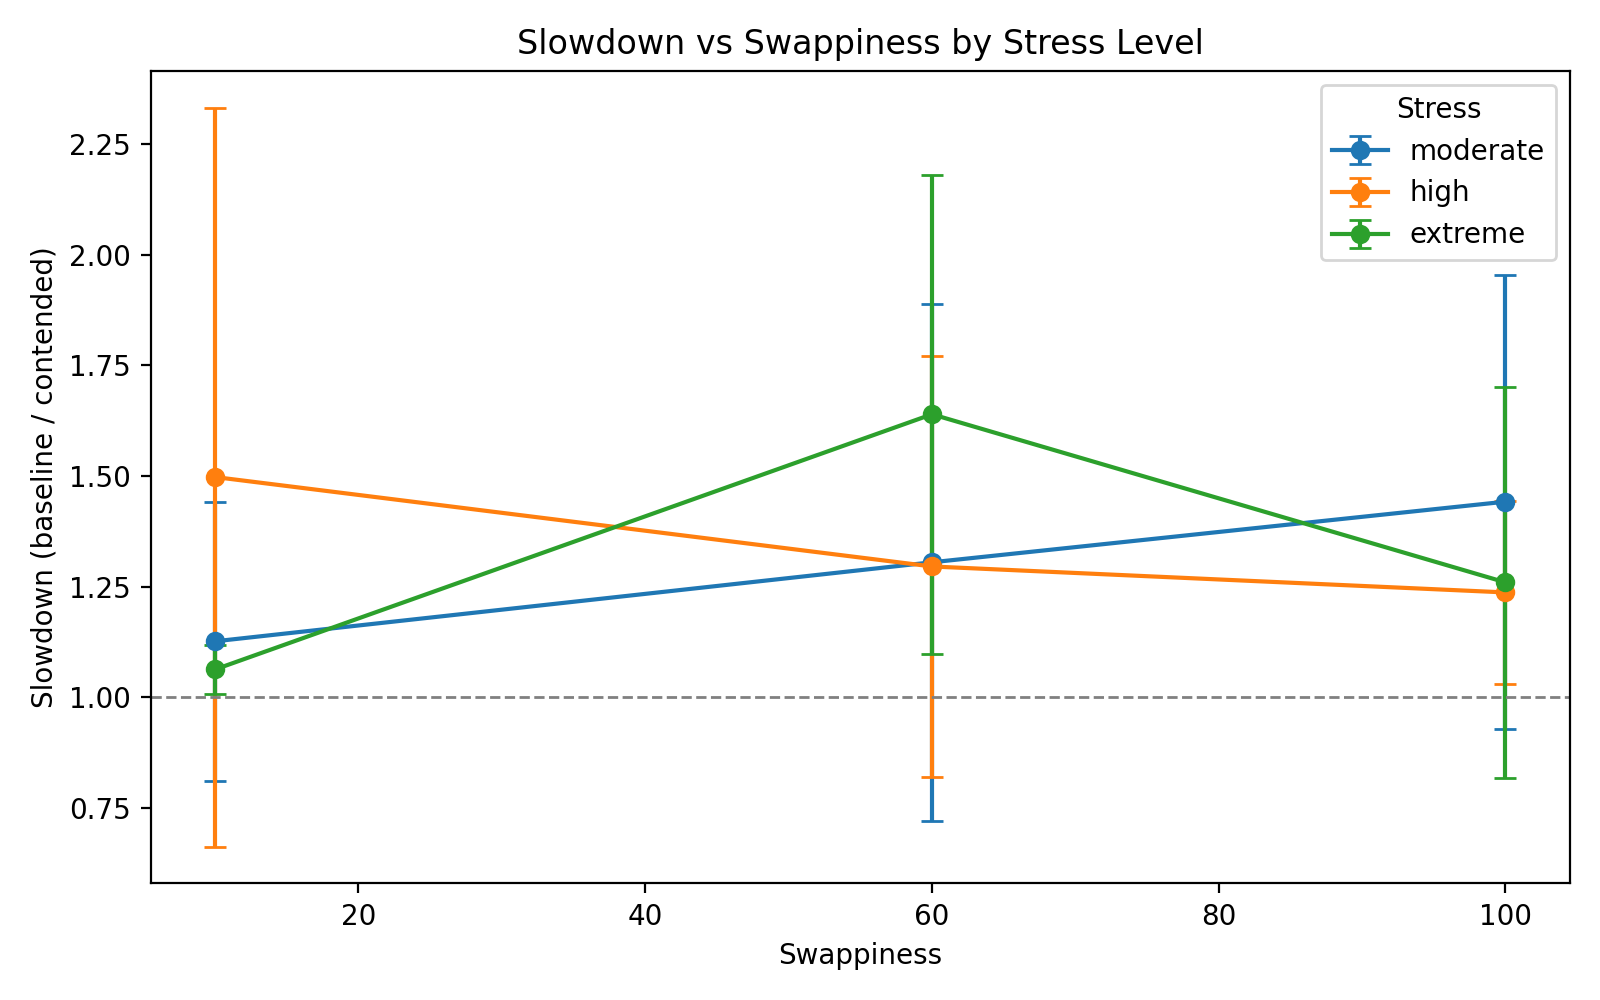
\includegraphics[width=0.95\columnwidth]{plots/slowdown_vs_swappiness.png}
  \caption{Mean slowdown versus swappiness for each stress level. Values above 1.0 indicate lower throughput than the baseline run.}
  \label{fig:docker-slowdown}
\end{figure}

\begin{figure}[t]
  \centering
  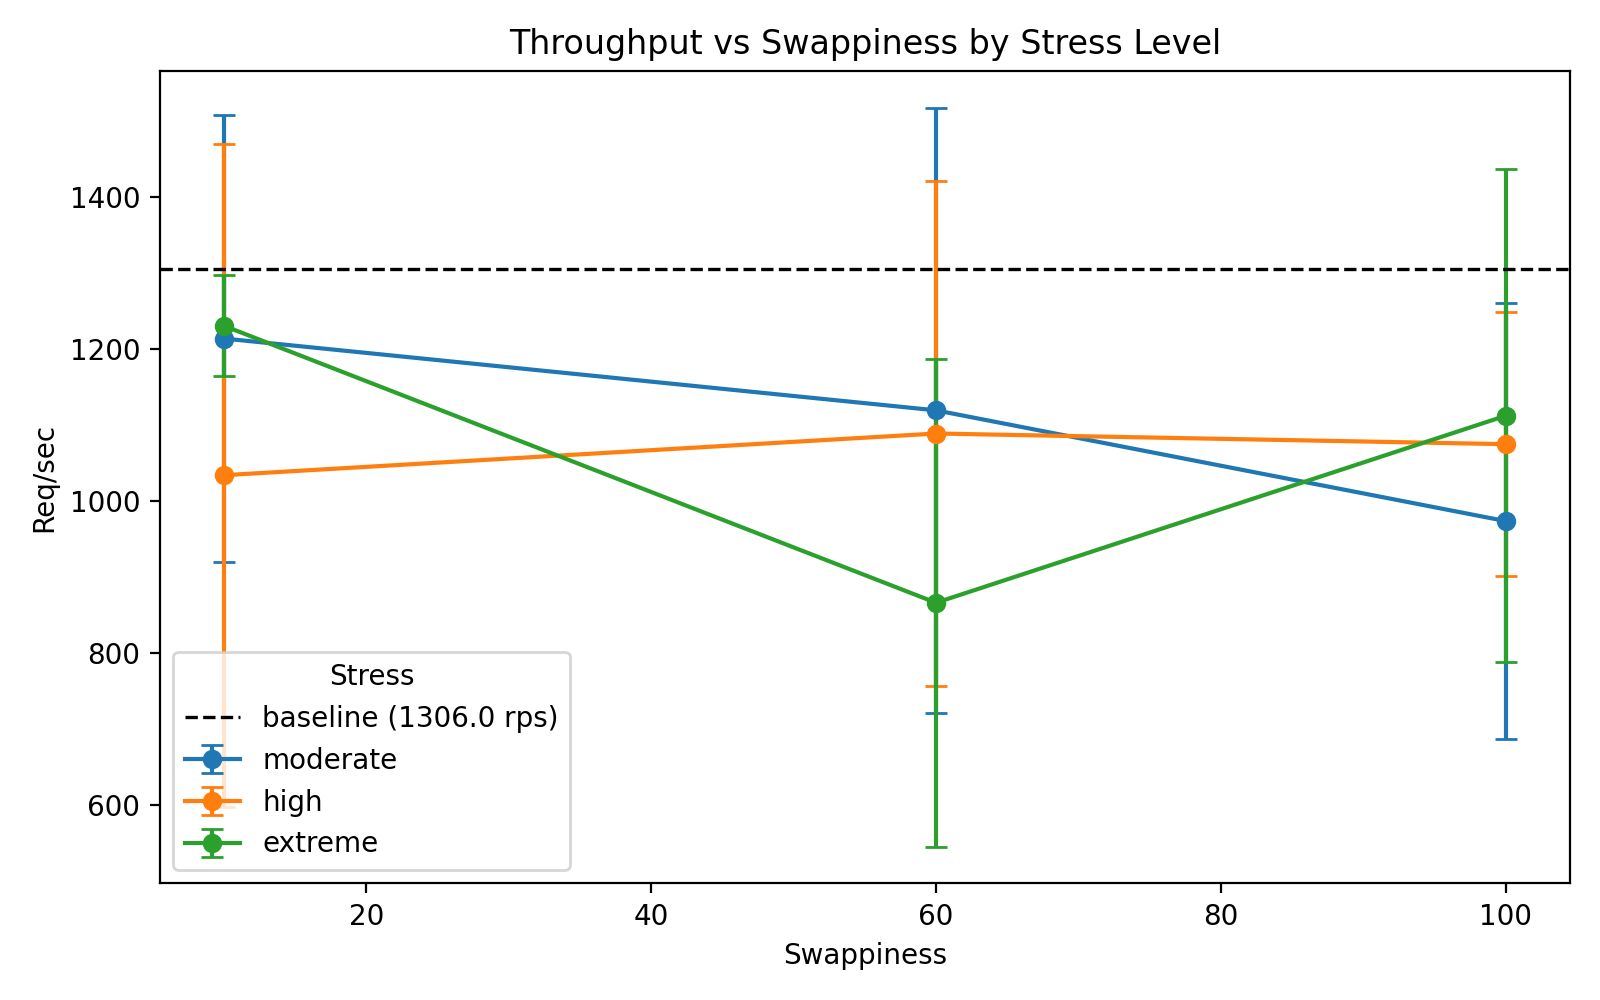
\includegraphics[width=0.95\columnwidth]{plots/throughput_vs_swappiness.png}
  \caption{Requests per second versus swappiness. The horizontal line marks the single global baseline throughput.}
  \label{fig:docker-throughput}
\end{figure}

\begin{figure}[t]
  \centering
  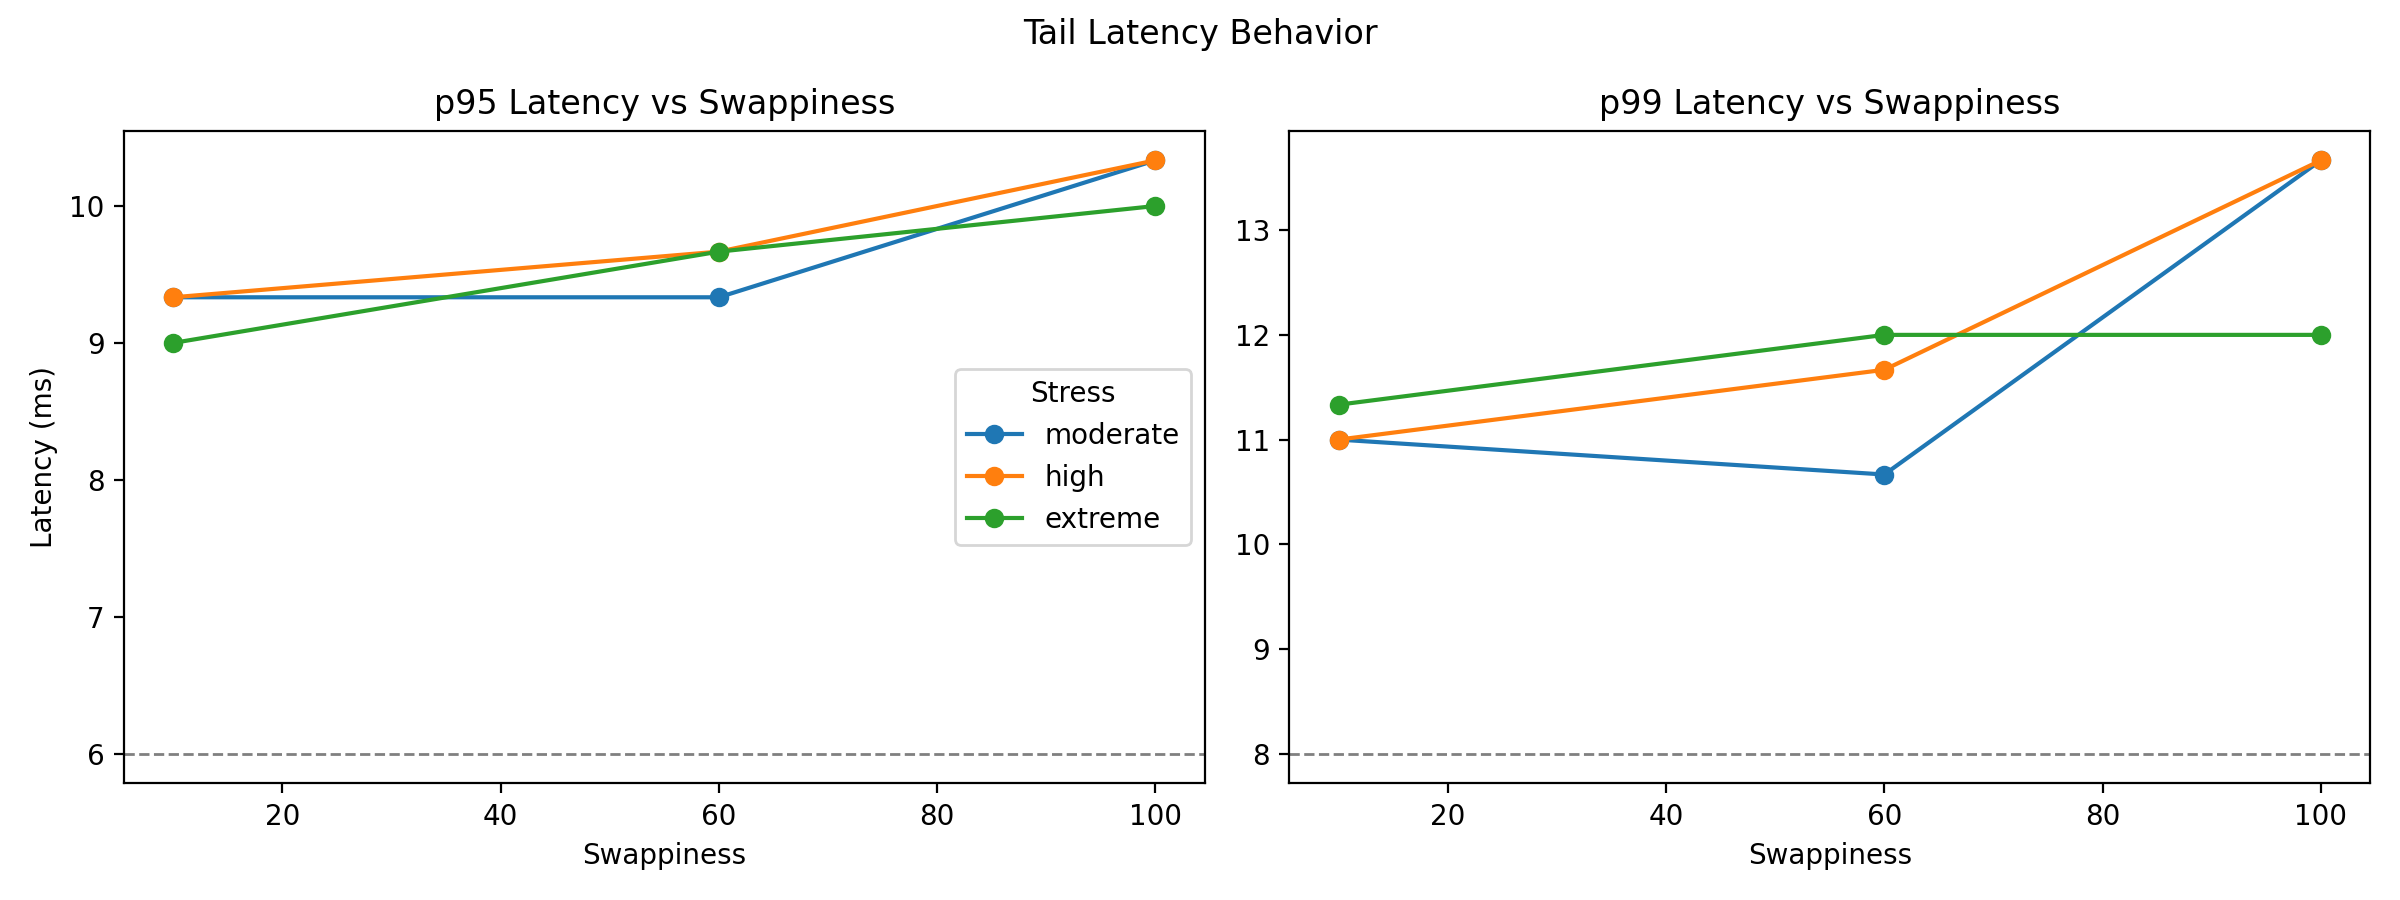
\includegraphics[width=0.95\columnwidth]{plots/tail_latency_vs_swappiness.png}
  \caption{Tail latency trends for p95 and p99 response times across swappiness values.}
  \label{fig:docker-tail}
\end{figure}

\begin{figure}[t]
  \centering
  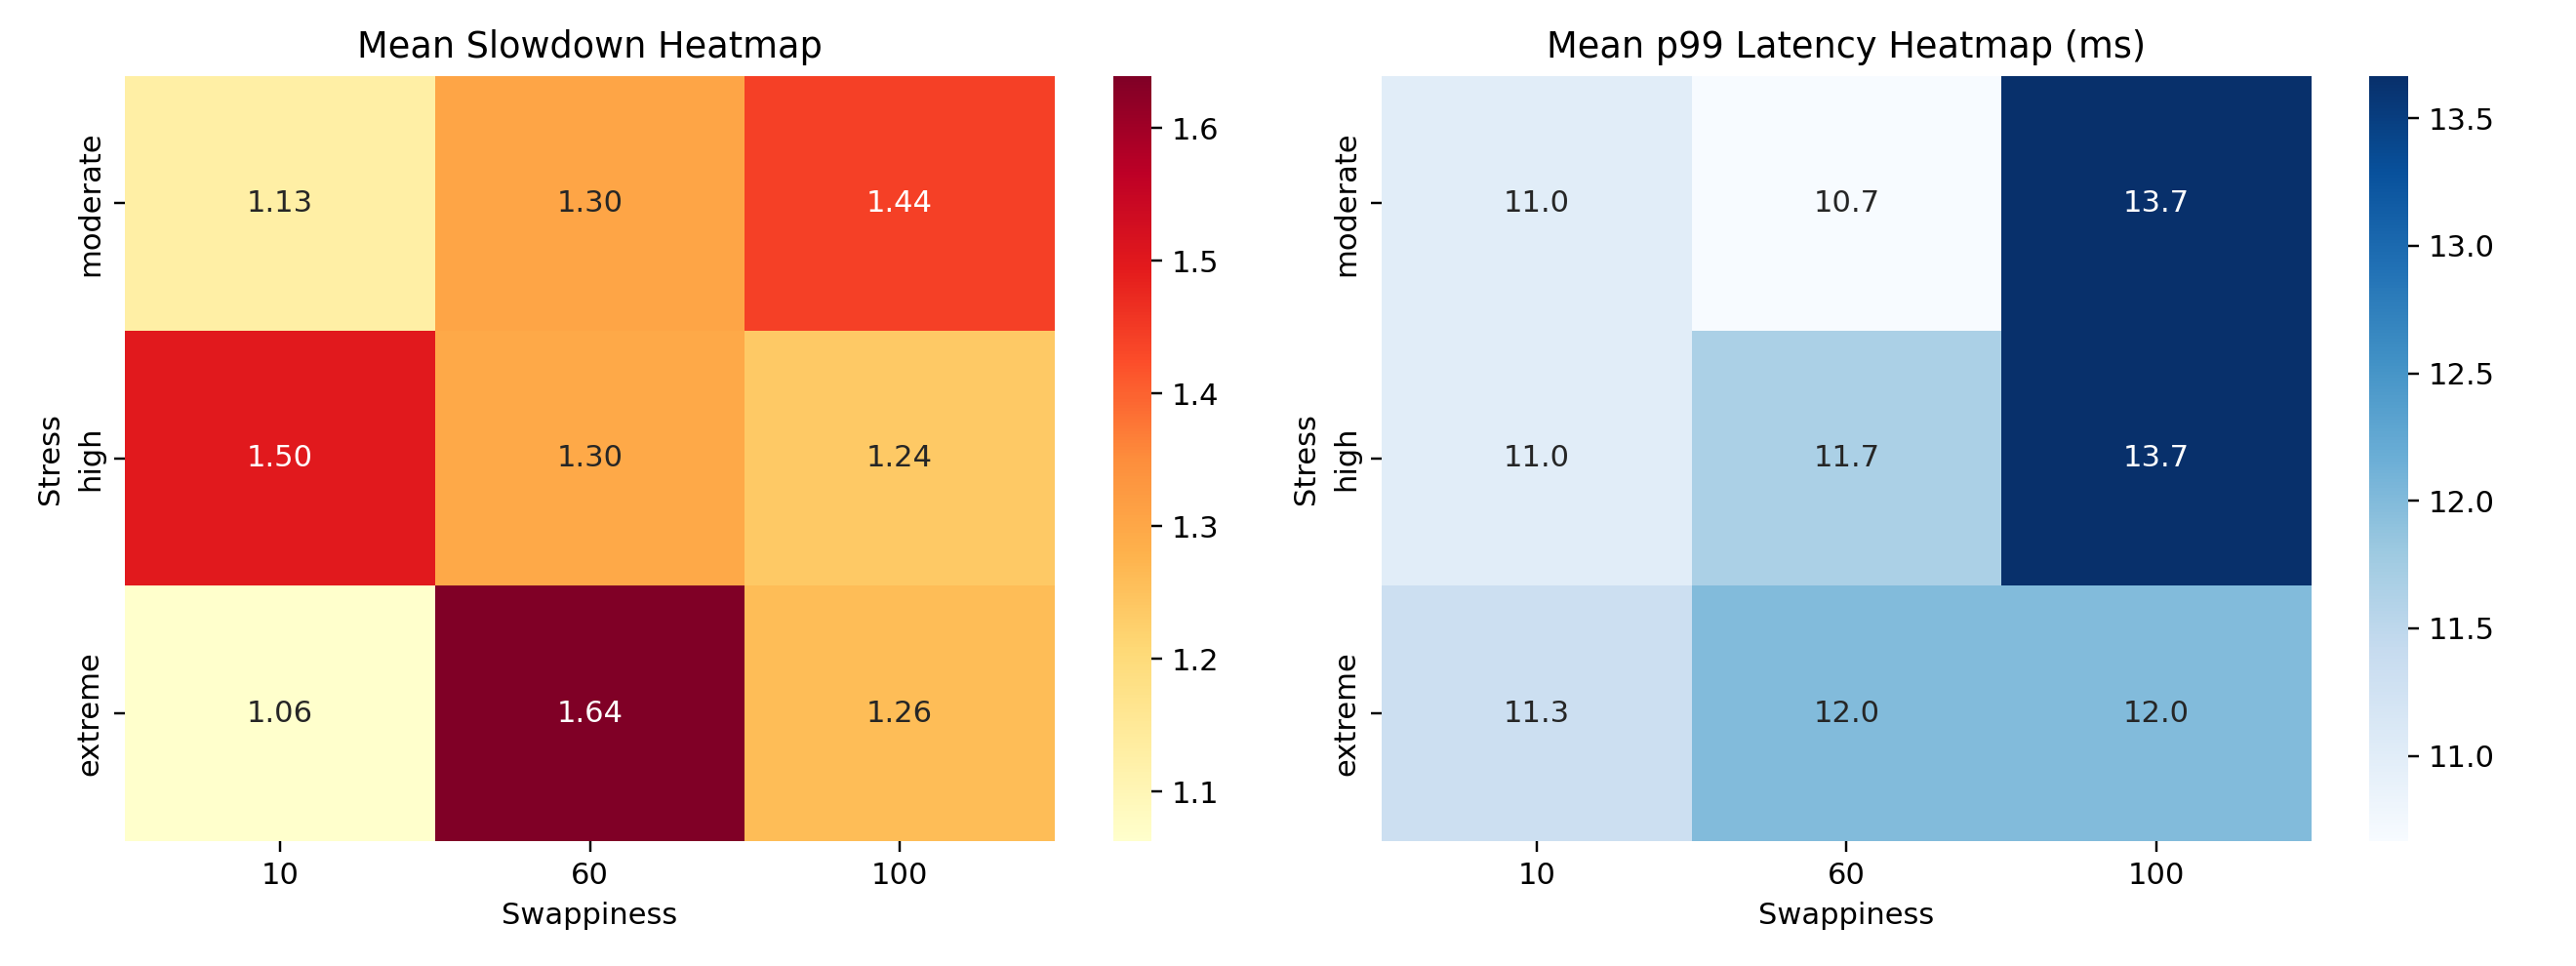
\includegraphics[width=0.95\columnwidth]{plots/heatmaps_slowdown_p99.png}
  \caption{Heatmaps of mean slowdown and mean p99 latency across the stress matrix.}
  \label{fig:docker-heatmap}
\end{figure}

The baseline achieved about 1306 requests/sec with p95 around 6 ms and p99 around 8 ms. Under contention, throughput generally decreased across stressed configurations, although some runs remained close to baseline due to run-to-run variability. The smallest slowdown was observed at swappiness 10 with extreme stress. The strongest degradation appeared at swappiness 60 with extreme stress. In the throughput plot, this appears as an overall reduction relative to the baseline, although the trend is not strictly monotonic across swappiness levels.

Across the stressed runs, p95 latency clustered around 9--10 ms and p99 latency around 11--14 ms, which is higher than the baseline tail latency. The tail-latency plot shows that the effect is not isolated to a single stress level; instead, tail latency increased under memory pressure, with high-percentile response times elevated across the stress matrix.

The distribution across repeats indicates non-negligible variability. Some swappiness and stress combinations show larger spread in throughput and slowdown than others, which suggests that the system response is somewhat sensitive to run-to-run state such as cache warmth, reclaim timing, and container scheduling noise. A small number of runs also recorded request failures, which is consistent with transient instability under heavier contention.

Kernel counters were less dramatic than the application-level metrics. Across all configurations, swap activity remained minimal, indicating that performance degradation was not driven by sustained disk-backed paging \cite{nakazawa2017taming}. Instead, the performance impact is more visible in throughput loss, tail-latency inflation, and occasional request failures.

\subsection{KVM Experiments}

The KVM campaign followed the same experimental matrix as the Docker setup, with a single global baseline at swappiness 60 and ApacheBench concurrency fixed at 30. Each stressed configuration was repeated three times, and results were aggregated for analysis. The most relevant plots are shown in Figures~\ref{fig:kvm-slowdown}, \ref{fig:kvm-throughput}, \ref{fig:kvm-tail}, and \ref{fig:kvm-heatmap}.

\begin{figure}[t]
  \centering
  
\includegraphics[width=0.95\columnwidth]{kvm_plots/kvm_slowdown_vs_swappiness.png}
  \caption{Mean slowdown versus swappiness for KVM experiments.}
  \label{fig:kvm-slowdown}
\end{figure}

\begin{figure}[t]
  \centering
  
\includegraphics[width=0.95\columnwidth]{kvm_plots/kvm_throughput_vs_swappiness.png}
  \caption{Throughput (requests/sec) versus swappiness for KVM.}
  \label{fig:kvm-throughput}
\end{figure}

\begin{figure}[t]
  \centering
  
\includegraphics[width=0.95\columnwidth]{kvm_plots/kvm_tail_latency_vs_swappiness.png}
  \caption{Tail latency (p95 and p99) across swappiness values in KVM.}
  \label{fig:kvm-tail}
\end{figure}

\begin{figure}[t]
  \centering
  
\includegraphics[width=0.95\columnwidth]{kvm_plots/kvm_heatmaps_slowdown_p99.png}
  \caption{Heatmaps of slowdown and p99 latency across KVM stress configurations.}
  \label{fig:kvm-heatmap}
\end{figure}

The baseline throughput for the KVM environment was approximately 1420 requests/sec with p95 latency around 5 ms and p99 latency around 6 ms. Compared to the Docker baseline, the VM baseline performance is similar in magnitude, which is consistent with prior studies showing near-native performance for virtual machines under non-contended conditions \cite{felter2015comparison}.

Under memory pressure, the degradation patterns differ from the Docker results. Across all configurations, the mean slowdown ranges from approximately 0.89x to 1.26x relative to baseline. In several configurations, particularly at swappiness 60 and moderate-to-high stress, throughput slightly improves relative to the baseline, which results in slowdown values below 1.0. This effect is likely due to reduced interference or measurement noise rather than a true performance gain.

The highest mean slowdown is observed at swappiness 100 under high stress ($\approx$ 1.26×), although this configuration also exhibits high variability, indicating unstable performance rather than consistently poor behavior.

Tail latency remains relatively stable compared to the Docker results, with only modest variation across swappiness and stress levels. The p95 latency is generally between 4--5.3 ms, and p99 latency remains between 5--7.7 ms for most configurations. Compared to the Docker results, tail latency inflation is smaller and more consistent across stress levels.

Kernel-level metrics show minimal swap activity and very low major page fault counts in most runs. The absence of significant swap-in and swap-out activity suggests that performance degradation is not dominated by sustained disk-backed paging in the observed configurations.

As in the container experiments, varying swappiness did not result in sustained swap activity, suggesting that reclaim behavior dominates performance effects in the evaluated configurations.

Variability across runs is present but lower than in the Docker experiments for most configurations, except for the swappiness 100 high-stress case. This suggests that the VM environment is more stable under moderate and high pressure. Instability appears primarily under aggressive reclaim configurations.

An important observation is that configurations with swappiness 60 consistently show slowdown values below or close to 1.0 across stress levels, indicating that moderate reclaim aggressiveness may help maintain stable performance in the VM environment.

\subsection{Fairness Analysis}

Although Jain’s Fairness Index was initially considered as a metric, the analysis showed that it does not reveal significant differences across the tested configurations. For completeness, we report the results for the Docker experiments: the fairness index remains high, ranging from approximately 0.95 to 0.99 across swappiness and stress levels. This indicates that memory pressure does not create strong imbalance between the latency-sensitive service and the stress workload.

We include these results to provide a complete view of the system behavior, but note that they do not materially affect the conclusions drawn from throughput, slowdown, or tail-latency metrics. The overall variation in fairness is minor, suggesting that performance degradation under memory pressure is largely uniform across competing workloads.

\subsection{Failure and Re-run Observations}

During the experimental campaign, a small number of runs experienced transient failures, primarily in the form of socket connection resets during ApacheBench execution. These failures occurred under higher memory pressure configurations and required rerunning those experiments to obtain valid measurements.

These events are not treated as experimental errors but rather as indicators of system instability under stress. In particular, connection resets suggest that memory pressure may impact not only application performance but also network stack responsiveness and system-level reliability.

Therefore, these observations are treated as part of normal system behavior under extreme memory pressure rather than as outliers.

\section{Discussion}

\subsection{Docker Experiments}

The Docker results support the interpretation that memory pressure degrades application performance even when the service remains available. The clearest signal is the reduction in throughput and the increase in tail latency under all stressed configurations. That pattern is consistent with the service container competing with the stress container for memory and reclaim bandwidth, even though the host-level swap counters did not show large sustained activity in most runs \cite{nakazawa2017taming}.

From a systems perspective, the results suggest that contention in a shared-kernel environment shows up first as responsiveness loss \cite{dean2013tail} rather than catastrophic failure. The service continues to run, but the higher-percentile response times increase and throughput becomes less stable. This is important for latency-sensitive workloads because tail latency is often more visible to users than average throughput \cite{dean2013tail}.

The swappiness setting influenced the results, but not in a perfectly monotonic way. Some configurations at swappiness 60 performed worse than the lower or higher values, and the variance across repeats indicates that the system is near a regime where reclaim behavior is sensitive to runtime state \cite{mars2011bubble}. That makes it risky to make a simple claim that one swappiness value is always best for all pressure levels. A safer interpretation is that memory pressure and kernel reclaim policy interact in a non-linear way, and the best setting depends on the workload mix and stress intensity.

The occasional request failure is also meaningful. Even a single failed request under extreme contention is evidence that the benchmark is not merely slower but occasionally unstable. For the report, this should be described as observed interference under heavy memory pressure, not as proof that the kernel or container runtime is fundamentally broken. It is a symptom of the stress conditions you created.

Overall, these Docker results are consistent with the project goal: containers provide lightweight isolation, but shared-kernel memory contention still harms throughput, tail latency, and run-to-run stability \cite{bhaia2024isolation}. The current dataset is strong enough to support a Docker results section and to motivate the KVM comparison, but it should avoid overclaiming swap-heavy behavior unless you add more runs that show stronger vmstat activity.

\subsection{KVM Experiments}

The KVM results show a different performance profile compared to the container-based experiments. The most important observation is that performance degradation under memory pressure is smaller and more stable in the VM environment.

Throughput degradation is limited in most configurations, and several cases even show apparent improvement relative to baseline. These improvements should not be interpreted as actual performance gains, but rather as artifacts of measurement variability, scheduling effects, or transient differences in system state. The key takeaway is that performance remains close to baseline for a large portion of the stress matrix.

Tail latency behavior further highlights the difference between the two environments. In contrast to the Docker results, where tail latency consistently increased under pressure, the KVM experiments show relatively stable p95 and p99 latency across all stress levels. This suggests that the VM environment is more effective at shielding latency-sensitive workloads from interference caused by competing memory-intensive tasks.

From a systems perspective, this behavior can be explained by the stronger isolation boundary provided by virtualization \cite{felter2015comparison, WaldspurgerProceedingsOT}. Because each workload runs inside a separate guest operating system with dedicated memory allocation, contention is largely confined within the VM. The host kernel does not directly mediate memory competition between the service and the stress workload, which reduces cross-workload interference.

Another important observation is the lack of significant swap activity and major page faults in the collected metrics. This indicates that the guest operating system manages memory pressure internally without triggering heavy disk-backed paging. As a result, the system avoids the large latency penalties typically associated with swapping \cite{dean2013tail}.

However, the results also show that instability can still occur under certain configurations. The swappiness 100 high-stress case exhibits high variability in throughput and slowdown, indicating that aggressive reclaim policies can still introduce unpredictability. This suggests that while virtualization improves isolation, it does not eliminate the impact of poor memory management parameter choices.

Overall, the KVM results support the interpretation that virtual machines provide stronger isolation under memory pressure, resulting in more stable throughput and tail latency compared to containers. The trade-off is that this stability comes from isolating workloads within fixed memory boundaries, which limits direct competition but may also restrict flexibility in memory utilization.

These findings align with the broader expectation that containers prioritize efficiency and resource sharing, while virtual machines prioritize isolation and predictability. The combined results from Docker and KVM experiments highlight this fundamental trade-off and provide empirical evidence of how it manifests under controlled memory pressure conditions.

\subsection{Comparative Analysis: Containers vs Virtual Machines}
We now directly compare the behavior of container-based and virtualized environments under equivalent memory pressure conditions. A direct comparison of the Docker and KVM results reveals clear differences in how the two virtualization approaches respond to similar memory pressure conditions.

The most significant difference lies in \textbf{performance degradation patterns}. In the Docker experiments, memory pressure consistently led to throughput reduction and increased tail latency across all stress levels. In contrast, the KVM experiments show much smaller degradation, with several configurations remaining close to baseline performance and exhibiting only mild slowdown.

This difference can be attributed to differences in the \textbf{memory isolation model} \cite{linux_cgroup_memory_controller}. In Docker, containers share the host kernel and page cache, which means that memory reclaim decisions are made globally across all workloads. As a result, the latency-sensitive service directly competes with the stress workload for memory and reclaim bandwidth. This leads to interference effects such as increased tail latency and reduced throughput.

In contrast, KVM provides \textbf{stronger isolation through separate guest operating systems}. Each VM operates within its own memory allocation, and memory pressure is largely handled internally by the guest OS \cite{kivity2007kvm , WaldspurgerProceedingsOT}. This prevents direct cross-workload interference at the host kernel level, which explains the more stable throughput and tail latency observed in the KVM results.

Another key difference is observed in \textbf{tail latency sensitivity}. The Docker experiments show consistent inflation of p95 and p99 latency under memory pressure, indicating that reclaim activity introduces delays visible at the application level. In the KVM experiments, tail latency remains relatively stable across most configurations. This suggests that virtualization is more effective at shielding latency-sensitive workloads from memory contention effects.

\textbf{Variability and predictability} also differ between the two environments. Docker results exhibit higher run-to-run variability, particularly under extreme stress, which indicates sensitivity to reclaim timing and shared-kernel state. KVM results are generally more stable, with lower variance except in the most aggressive configurations (e.g., swappiness 100 under high stress). This suggests that virtualization improves performance predictability under moderate pressure.

Importantly, neither environment shows strong evidence of sustained swap-driven degradation in the current dataset. Kernel metrics confirm that swap activity remains minimal in both environments, indicating that reclaim dominates performance degradation rather than disk paging.

A critical observation across both environments is the occurrence of \textbf{transient request failures}, including socket connection resets during some high-pressure runs. These failures required rerunning certain configurations to obtain complete datasets. While not frequent, these events are important because they indicate that memory pressure can push the system into unstable regimes where network-level errors occur. Rather than being treated as noise, these failures should be interpreted as evidence of system stress and degraded quality of service under extreme conditions.

Overall, the comparative results highlight a fundamental trade-off:

\begin{itemize}
\item \textbf{Containers (Docker):} higher efficiency and flexibility, but increased susceptibility to interference under memory pressure due to shared kernel resources.
\item \textbf{Virtual Machines (KVM):} stronger isolation and more stable performance under pressure, at the cost of fixed memory allocation and reduced resource sharing.
\end{itemize}

These findings demonstrate that the choice between containers and virtual machines should depend on workload characteristics. Latency-sensitive and performance-critical applications may benefit from the stronger isolation of VMs, while throughput-oriented or resource-efficient deployments may favor containers despite their higher sensitivity to memory contention.

\section{Threats to Validity}

Several factors may influence the interpretation of the results in this study.

First, the experiments are conducted on a single hardware platform with a specific CPU and memory configuration. Results may vary on systems with different hardware characteristics, particularly under different memory capacities or storage performance.

Second, the workload used in this study is a simplified HTTP service benchmark. While ApacheBench provides controlled and repeatable measurements, real-world applications may exhibit different memory access patterns and sensitivity to memory pressure.

Third, the VM configuration uses a fixed memory allocation without explicitly enabling advanced hypervisor features such as ballooning. As a result, the observed behavior primarily reflects guest-level memory management rather than full host-guest interaction.

Fourth, while multiple repetitions are used to reduce variability, some configurations exhibit run-to-run fluctuations. Factors such as cache state, scheduling effects, and background system activity may influence results.

Finally, swap activity was minimal in the observed experiments, which limits conclusions about swap-heavy scenarios. Additional experiments with stronger overcommitment or different storage configurations may be required to fully characterize swap-driven behavior.

Despite these limitations, the controlled experimental design and consistent trends across configurations provide confidence in the observed comparative behavior between containers and virtual machines under memory pressure.

\section{Conclusion}

This paper presented a systematic experimental study of how memory pressure affects performance and isolation in container-based and virtualized environments. Using controlled stress scenarios, we compared Docker containers and KVM virtual machines across multiple pressure regimes, focusing on throughput, tail latency, and performance degradation.

The results demonstrate that memory pressure degrades performance in both environments, but the impact differs significantly due to their underlying isolation mechanisms.

In container-based environments, memory pressure leads to higher throughput degradation, significant increases in tail latency, and greater run-to-run variability. These effects arise from shared-kernel resource contention, where workloads compete for memory and reclaim bandwidth. Even in the absence of heavy swap activity, reclaim behavior introduces latency spikes and performance instability.

In contrast, virtual machine environments exhibit more stable throughput, minimal impact on tail latency, and stronger isolation under comparable pressure conditions. Because memory contention is largely confined within the guest operating system, interference between workloads is reduced. However, performance sensitivity to aggressive reclaim policies indicates that isolation does not fully eliminate the effects of memory pressure.

A key finding across both environments is that performance degradation is primarily driven by memory reclaim rather than sustained swapping \cite{nakazawa2017taming}. Additionally, transient failures observed under extreme pressure suggest that memory contention can affect not only performance but also system stability.

Overall, the study highlights a fundamental trade-off: containers prioritize efficiency and flexible resource sharing but are more susceptible to contention, while virtual machines provide stronger isolation and more predictable performance at the cost of reduced flexibility.

\section{Future Work}

This work can be extended in several directions to further understand memory pressure behavior in virtualized systems.

First, future experiments could explore more aggressive overcommitment scenarios to analyze swap-heavy behavior and its impact on performance and tail latency. Additionally, enabling hypervisor-level mechanisms such as memory ballooning would allow investigation of guest-host memory management interactions and their role in mitigating double paging.

Second, the experimental design can be expanded to include multi-VM scenarios, where multiple virtual machines compete for host resources. This would provide a more realistic representation of cloud environments and enable deeper analysis of cross-VM interference.

Third, incorporating real-world workloads with diverse memory access patterns would improve the external validity of the results. Applications such as databases or in-memory caches may exhibit different sensitivity to memory pressure compared to the synthetic workloads used in this study.

Finally, future work could refine fairness analysis by exploring more sensitive metrics or workload configurations that better capture imbalance under contention, as the current results show limited variation in fairness across scenarios.

\bibliographystyle{IEEEtran}
\bibliography{references}
\end{document}
